%----------------------------------------------------------------------------------------
%	SECTION 1
%----------------------------------------------------------------------------------------

\section{Geometric Representations of Matroids of Small Rank.}

\begin{definition}
    Let $V$ be a vector space over a field $F$ of dimension $m$, a set of
    vector $\{v_1, \dots, n_k\}$, not all necessarily distinct, is called
    \textbf{affinely dependent} if there exists scalars $a_1, \dots, a_k \in F$,
    not all $0$ such that
    \begin{equation*}
        a_1v_1+\dots+a_kv_k=0
    \end{equation*}
    and
    \begin{equation*}
        a_1+\dots+a_k=0
    \end{equation*}
    We call $\{v_1, \dots, v_k\}$ \textbf{affinely independent} if they are not
    affinely dependent.
\end{definition}

We present one lemma on affine independence without proof.

\begin{lemma}\label{1.5.1}
    A set $\{v_1, \dots. v_k\}$ of vectors (not necesarily distinct) of a
    vector space $V$ of dimension $m$ is affinely dependent if the set of
    vectors $\{(1,v_1), \dots, (1,v_k))\}$ is linearly dependent in the vector
    space $F^{m+1}$.
\end{lemma}
\begin{corollary}
    $\{v_1, \dots, v_k\}$ is affinely independent if $\{(1,v_1), \dots,
    (1,v_k))\}$ is linearly independent.
\end{corollary}

\begin{lemma}\label{1.5.2}
    Let $V$ be a vector space of dimension $m$ over a field $F$, and let  $E$
    be the set of vectors of $V$, not all necesarily distinct. If $\Ic$ is the
    collection of all subsetets of  $E$ which are affinely independent, then
    $E$ together with  $\Ic$ forms a matroid.
\end{lemma}
\begin{proof}
    By lemma \ref{1.5.1}, we have that $M=M[A]$ where $A$ is the  $(m+1) \times
    n$ matrix over $F$ whose columns are  $(1,v_i)^T$.

    Alternatively, if we prove this directly by definition, we see that
    $\emptyset \in \Ic$, since  $\emptyset$ is affinely independent. Moreover,
    if  $\{v_1, \dots, v_k\}$, is affinely independent, then
    $a_1v_1+\dots+a_kv_k$ with $a_1+\dots+a_k=0$ implies that $a_i=0$ for each
    $1 \leq i \leq k$, then indexing  $1 \leq j \leq i$, we get that the subset
    $\{u_1, \dots, u_j\}$ of $\{v_1, \dots, v_k\}$ is also affinely independnet.

    Now suppose that $U=\{u_1, \dots, u_k\}$, and $V=\{v_1, \dots, v_n\}$ are
    affinely independnet, with $k>n$, so that  $|U|<|V|$. Then by definition, we
    have that
    \begin{align*}
        a_1v_1+\dots+a_kv_k=0,  &&   a_1+\dots+a_k=0 \\
    \end{align*}
    implies $a_i=0$ for ech $1 \leq i \leq k$, and
    \begin{align*}
        b_1u_1+\dots+b_nu_n=0,  &&  b_1+\dots+b_n=0
    \end{align*}
    implies $b_j=0$ for ech $1 \leq j \leq n$

    Then choose a vector $v_i \in \com{V}{U}$, so that $v_i \neq u_j$ for all
    $u_j$ of  $U$. Then we find that:
    \begin{align*}
        (b_1u_1+\dots+b_nu_n)+a_iv_i=0,  &&  (b_1+\dots+b_n)+a_i=0
    \end{align*}
    Since $v_i \in V$,  $a_i=0$, so that the set  $U \cup v_i$ is also affinely
    independent. Therefore $E$ forms a matroid having  $\Ic$ as its collection
    of independent sets.
\end{proof}

\begin{example}\label{1.17}
    Let $E=\{(0,0), (1,0), (2,0), (0,1), (0,2), (1,1)\}$ Of $\R^2$, and consider
    the affine matroid on $E$ We find that this matroid can be represented by
    the geometric figure in figure \ref{fig_1.9} below.
    \begin{figure}[h]
        \centering
        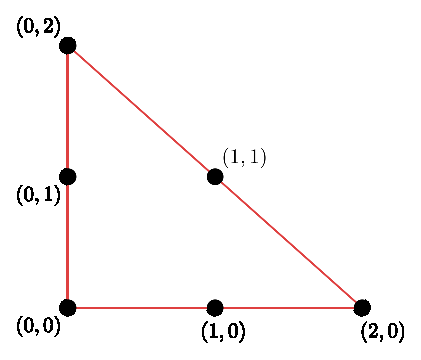
\includegraphics[scale=0.8]{Figures/Chapter1/rank_3_affine_matroid.eps}
        \caption{An affine matroid of rank $3$.}
        \label{fig_1.9}
    \end{figure}
\end{example}
